\documentclass[aspectratio=169,11pt]{beamer}
\usepackage[T1]{fontenc}
\usepackage{lmodern}
\usepackage{amsmath,amssymb,booktabs,listings,array}
\usetheme{Madrid}
\usecolortheme{dolphin}
\setbeamertemplate{blocks}[rounded][shadow=false]
\definecolor{Navy}{HTML}{15345C}
\definecolor{Teal}{HTML}{2266B3}
\definecolor{Coral}{HTML}{D6603C}
\definecolor{Mist}{HTML}{EFF5FC}
\setbeamercolor{normal text}{fg=Navy,bg=white}
\setbeamercolor{structure}{fg=Teal}
\setbeamercolor{frametitle}{fg=white,bg=Navy}
\setbeamercolor{title}{fg=white,bg=Navy}
\setbeamercolor{subtitle}{fg=white}
\setbeamercolor{alerted text}{fg=Teal}
\setbeamercolor{palette primary}{fg=white,bg=Teal}
\setbeamercolor{palette secondary}{fg=white,bg=Navy}
\setbeamercolor{palette tertiary}{fg=white,bg=Navy}
\setbeamercolor{block title}{fg=white,bg=Teal}
\setbeamercolor{block body}{fg=Navy,bg=Mist}
\setbeamerfont{title}{size=\Huge,series=\bfseries}
\setbeamerfont{frametitle}{size=\Large,series=\bfseries}
\setbeamertemplate{navigation symbols}{}
\setbeamertemplate{itemize items}[circle]
\setbeamersize{text margin left=9mm,text margin right=9mm}
\setbeamertemplate{headline}{}
\setbeamertemplate{footline}{%
 \leavevmode\hbox{%
 \begin{beamercolorbox}[wd=.84\paperwidth,ht=2.8ex,dp=1.2ex,leftskip=9mm]{palette secondary}%
 \scriptsize DRP\enspace\textbar\enspace Wasserstein Distance
 \end{beamercolorbox}%
 \begin{beamercolorbox}[wd=.16\paperwidth,ht=2.8ex,dp=1.2ex,center]{palette primary}%
 \scriptsize\insertframenumber\,/\,\inserttotalframenumber
 \end{beamercolorbox}}}
\lstset{language=Python,basicstyle=\ttfamily\small,keywordstyle=\color{Teal}\bfseries,
 stringstyle=\color{Coral},showstringspaces=false,columns=fullflexible,keepspaces=true,
 frame=none,backgroundcolor=\color{Mist},xleftmargin=2mm,xrightmargin=2mm,
 aboveskip=3mm,belowskip=3mm,breaklines=false}
\newcommand{\src}[2]{\vfill{\tiny\color{gray}\href{#1}{#2}}}
\newcommand{\otref}{\src{https://arxiv.org/abs/1803.00567}{Peyr\'e and Cuturi, Computational Optimal Transport, Sections 2--4.}}
\newcommand{\fig}[2][.95]{\begin{center}\includegraphics[width=#1\textwidth,height=.55\textheight,keepaspectratio]{figures/#2.pdf}\end{center}}
\title{Wasserstein distance}
\subtitle{Moving probability mass: formulas, computation, and data examples}
\author{\texorpdfstring{Directed Reading Program\\Florida State University}{Directed Reading Program, Florida State University}}
\date{}
\begin{document}

% 1
\begin{frame}
\titlepage
\end{frame}

% 2
\begin{frame}{Point masses: what do $\delta_0$ and $\delta_a$ mean?}
A probability distribution assigns a total mass of $1$ to possible outcomes.
\vspace{3mm}
\begin{itemize}\setlength\itemsep{3mm}
\item $P=\delta_0$ puts probability $1$ at position $0$. A sample from $P$ is always $0$.
\item $Q=\delta_a$ puts probability $1$ at position $a$. A sample from $Q$ is always $a$.
\item $a$ is a location, not an amount of probability. It can be negative.
\end{itemize}
\vspace{3mm}
For example, when $a=3$:
\begin{center}
\begin{tabular}{c cc}
\toprule
Position & Mass under $P$ & Mass under $Q$\\\midrule
$0$ & $1$ & $0$\\
$3$ & $0$ & $1$\\\bottomrule
\end{tabular}
\end{center}
The distance between the two locations is $|0-a|=|a|$.
\end{frame}

% 3
\begin{frame}{How to compute Wasserstein distance for discrete mass}
A \alert{transport plan} says how much probability to move from each source
position $x_i$ to each target position $y_j$. Call that amount $\pi_{ij}$.
\vspace{2mm}
\begin{enumerate}\setlength\itemsep{2mm}
\item Preserve the mass: send all source mass and fill each target's required mass.
\item For each move, multiply its mass by its distance raised to power $p$.
\item Add these costs, choose the cheapest valid plan, and take the $p$th root.
\end{enumerate}
\[
\boxed{W_p(P,Q)=\left(\min_{\text{valid plans }\pi}
\sum_{i,j}\underbrace{\pi_{ij}}_{\text{mass}}
\underbrace{|x_i-y_j|^p}_{\text{travel cost per unit mass}}\right)^{1/p}}
\]
Here $1\leq p<\infty$. For $W_1$, use distances. For $W_2$, use squared
distances, then take a square root.
\otref
\end{frame}

% 4
\begin{frame}{Computing $W_p(\delta_0,\delta_a)$}
There is only one valid plan: move all $1$ unit of mass from $0$ to $a$.
\vspace{3mm}
\[
\text{Total cost}=\underbrace{1}_{\text{mass}}\times
\underbrace{|0-a|^p}_{\text{cost per unit mass}}=|a|^p.
\]
\[
\boxed{W_p(\delta_0,\delta_a)=\bigl(|a|^p\bigr)^{1/p}=|a|}
\]
\vspace{3mm}
For $a=3$, the two most common choices give
\[W_1=1\times3=3,\qquad W_2=\sqrt{1\times3^2}=3.\]
For $a=-3$, both still equal $3$. For $a=0$, both equal $0$.\\[3mm]
The absolute value appears because travel distance is nonnegative.
\end{frame}

% 5
\begin{frame}{Total variation: comparing probabilities at each location}
For discrete distributions, use the convention
\[
\boxed{\operatorname{TV}(P,Q)=\frac12\sum_z
\left|P(\{z\})-Q(\{z\})\right|}.
\]
The sum runs over distinct locations. $P(\{z\})$ means the probability at $z$.
For $P=\delta_0$, $Q=\delta_a$, and $a\ne0$, only $0$ and $a$ contribute:
\[
\operatorname{TV}(P,Q)=\tfrac12\bigl(\underbrace{|1-0|}_{z=0}
+\underbrace{|0-1|}_{z=a}\bigr)=\boxed{1}.
\]
The factor $\tfrac12$ avoids counting the same missing mass twice.
\vspace{3mm}
\begin{itemize}\setlength\itemsep{2mm}
\item TV ranges from $0$ to $1$. Here the distributions have no shared mass.
\item Moving $a$ from $0.001$ to $100$ does not change those probability gaps.
\item If $a=0$, the distributions coincide and TV is $0$.
\end{itemize}
\end{frame}

% 6
\begin{frame}{KL divergence: a positive probability compared with zero}
For discrete distributions, write $p_z=P(\{z\})$ and $q_z=Q(\{z\})$:
\[
\boxed{D_{\rm KL}(P\Vert Q)=\sum_{z:p_z>0}p_z\log\frac{p_z}{q_z}}.
\]
If $p_z>0$ but $q_z=0$, that term is $+\infty$ by definition. The limiting
reason is $\log(1/\varepsilon)\longrightarrow+\infty$ as $\varepsilon\downarrow0$.
\vspace{3mm}
For $P=\delta_0$ and $Q=\delta_a$ with $a\ne0$:
\[p_0=1,\qquad q_0=0\qquad\Longrightarrow\qquad
\boxed{D_{\rm KL}(P\Vert Q)=+\infty}.\]
$P$ produces $0$ with certainty, while $Q$ assigns it zero probability.\\[3mm]
If $a=0$, the only term is $1\log(1/1)=0$.
KL is a divergence and is generally asymmetric.
\end{frame}

% 7
\begin{frame}{How the comparison changes as $a$ moves}
\small ``Discrepancy'' means a numerical measure of difference between distributions.
It is a general word, not a fourth formula. Each plot below names its measure.
\begin{center}
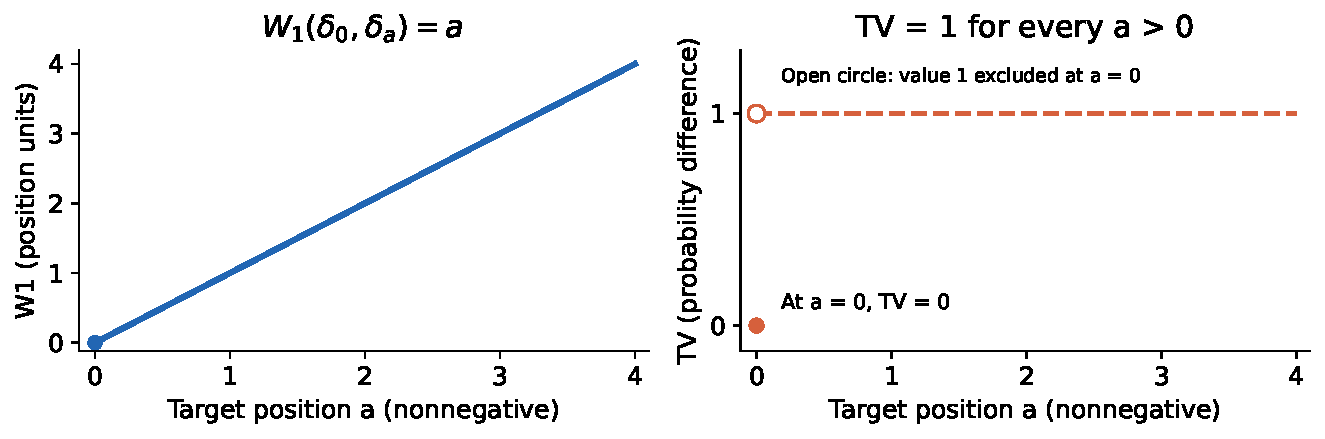
\includegraphics[width=.91\textwidth,height=.47\textheight,keepaspectratio]{figures/point_mass.pdf}
\end{center}
\small Each horizontal axis is the target position $a\geq0$, with $P=\delta_0$ fixed.\\[1mm]
$W_1$ measures travel in position units. TV measures probability difference.\\[1mm]
KL is $+\infty$ for every $a>0$, so it has no finite curve here.
At $a=0$, all three are $0$.
\otref
\end{frame}

% 8
\begin{frame}{The Wasserstein definition}
A \alert{coupling} $\pi\in\Pi(P,Q)$ is a joint distribution of $(X,Y)$ with marginals $P$ and $Q$.
\vspace{3mm}
\[\boxed{W_p(P,Q)=\left(\inf_{\pi\in\Pi(P,Q)}
\int d(x,y)^p\,d\pi(x,y)\right)^{1/p}},\qquad p\geq1.
\]
\begin{itemize}\setlength\itemsep{3mm}
\item $d(x,y)$ specifies the cost geometry between individual points.
\item We choose how to pair mass while preserving both distributions.
\item Assume finite $p$th moments. Then $W_p$ is a metric on these laws.
\end{itemize}
\vspace{2mm}
A plan can split mass. A deterministic map $Y=T(X)$ cannot split an atom.\\[2mm]
Independent pairing is feasible, but usually costs more than optimal pairing.
\otref
\end{frame}


% 9
\begin{frame}{A transport calculation by hand}
\[P=\tfrac12\delta_0+\tfrac12\delta_2,\qquad
Q=\tfrac14\delta_1+\tfrac34\delta_3\]
\begin{columns}
\begin{column}{.50\textwidth}
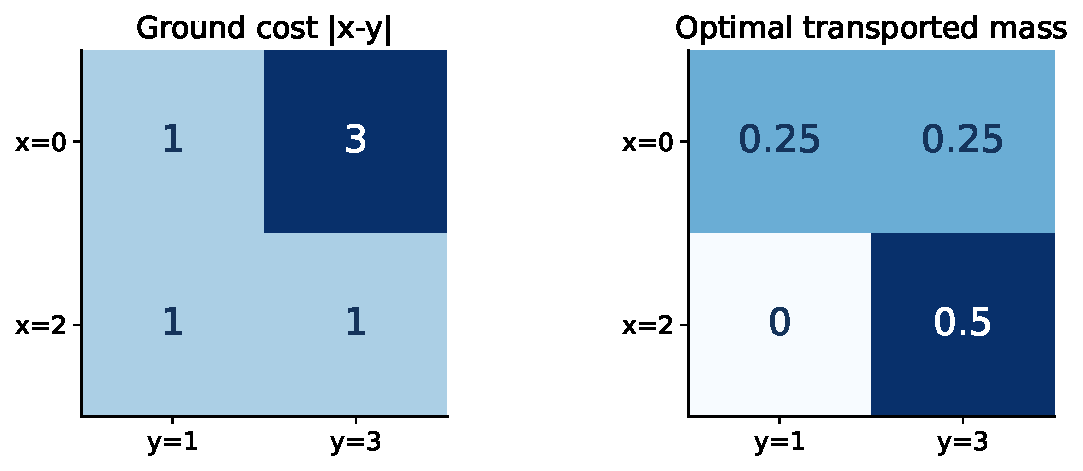
\includegraphics[width=\linewidth]{figures/discrete_plan.pdf}
\end{column}
\begin{column}{.48\textwidth}
Each entry $\pi_{ij}$ is an amount of mass.
\[W_1=\tfrac14(1)+\tfrac14(3)+\tfrac12(1)=1.5\]
\[W_2^2=\tfrac14(1^2)+\tfrac14(3^2)+\tfrac12(1^2)=3\]
\[W_2=\sqrt3\approx1.732\]
Row sums supply $P$. Column sums supply $Q$.
\end{column}
\end{columns}
\end{frame}

% 10
\begin{frame}{$W_1$ and $W_2$ measure different travel costs}
\begin{center}
\begin{tabular}{lll}
\toprule
& $W_1$ & $W_2$\\\midrule
Cost before optimization & $d(x,y)$ & $d(x,y)^2$\\[3mm]
Final operation & None & Square root\\[3mm]
Interpretation & Average travel & RMS travel\\[3mm]
Units & Same as $d$ & Same as $d$\\\bottomrule
\end{tabular}
\end{center}
\vspace{3mm}
$W_2$ gives more weight to large displacements. On the same metric space,
\[W_1(P,Q)\leq W_2(P,Q)\quad\text{when second moments are finite}.\]
\alert{A solver using squared ground costs returns $W_2^2$ before the square root.}
\otref
\end{frame}

% 11
\begin{frame}{In one dimension, equal quantiles match optimally}
\[W_p^p(P,Q)=\int_0^1\left|F_P^{-1}(u)-F_Q^{-1}(u)\right|^p\,du\]
\fig[.88]{quantiles}
\small For $W_1$, the area between CDFs also equals the distance:
$W_1=\int_{\mathbb R}|F_P(x)-F_Q(x)|\,dx$.
\otref
\end{frame}

% 12
\begin{frame}{An analytic formula for one-dimensional Gaussians}
\[P=\mathcal N(\mu_1,\sigma_1^2),\qquad Q=\mathcal N(\mu_2,\sigma_2^2)\]
Match quantiles using the same $Z\sim\mathcal N(0,1)$:
\[X=\mu_1+\sigma_1 Z,\qquad Y=\mu_2+\sigma_2 Z.\]
\begin{align*}
W_2^2(P,Q)&=\mathbb E\big[(\Delta\mu+\Delta\sigma Z)^2\big]\\
&=(\Delta\mu)^2+2\Delta\mu\Delta\sigma\underbrace{\mathbb E[Z]}_0
 +(\Delta\sigma)^2\underbrace{\mathbb E[Z^2]}_1.
\end{align*}
\[\boxed{W_2(P,Q)=\sqrt{(\mu_1-\mu_2)^2+(\sigma_1-\sigma_2)^2}}\]
\alert{The formula uses standard deviations.} A variance of $4$ means $\sigma=2$.
\otref
\end{frame}

% 13
\begin{frame}{Same variance, different means}
\begin{columns}
\begin{column}{.40\textwidth}
\[P=\mathcal N(0,1),\quad Q=\mathcal N(2,1)\]
Every quantile shifts right by $2$.
\[T(x)=x+2\]
\[\boxed{W_1=W_2=2}\]
The optimal transport is a translation.
\end{column}
\begin{column}{.58\textwidth}
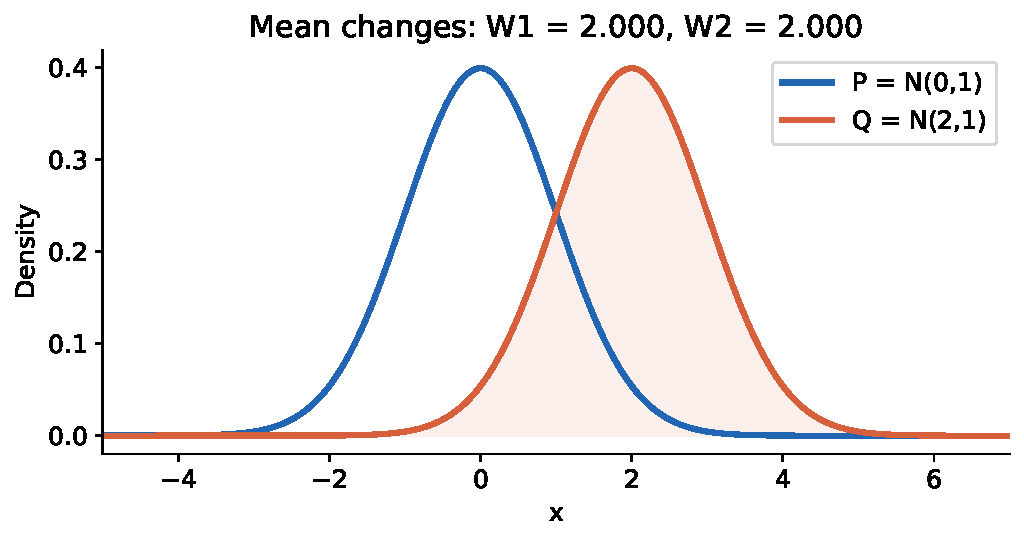
\includegraphics[width=\linewidth]{figures/gaussian_mean.pdf}
\end{column}
\end{columns}
\end{frame}

% 14
\begin{frame}{Same mean, different variances}
\begin{columns}
\begin{column}{.40\textwidth}
\[P=\mathcal N(0,1),\quad Q=\mathcal N(0,4)\]
The standard deviation changes from $1$ to $2$.
\[T(x)=2x\]
\[W_2=|2-1|=1\]
\[W_1=\mathbb E|Z|=\sqrt{2/\pi}\approx0.798\]
Equal means do not imply equal laws.
\end{column}
\begin{column}{.58\textwidth}
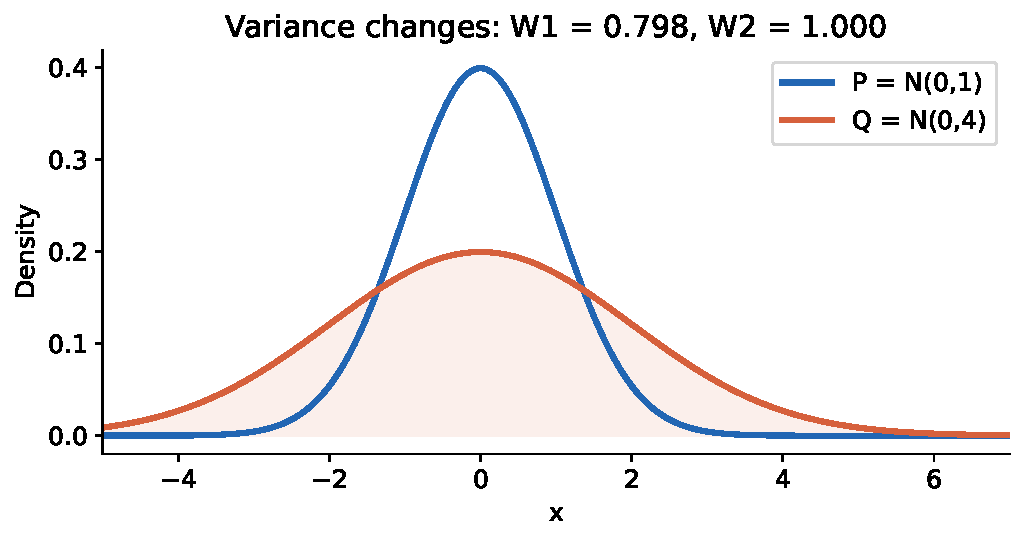
\includegraphics[width=\linewidth]{figures/gaussian_variance.pdf}
\end{column}
\end{columns}
\end{frame}

% 15
\begin{frame}{Both mean and variance change}
\begin{columns}
\begin{column}{.40\textwidth}
\[P=\mathcal N(0,1),\quad Q=\mathcal N(2,4)\]
\[T(x)=2+2x\]
\[W_2=\sqrt{2^2+(2-1)^2}=\sqrt5\]
\[W_1=\mathbb E|2+Z|\approx2.017\]
\end{column}
\begin{column}{.58\textwidth}
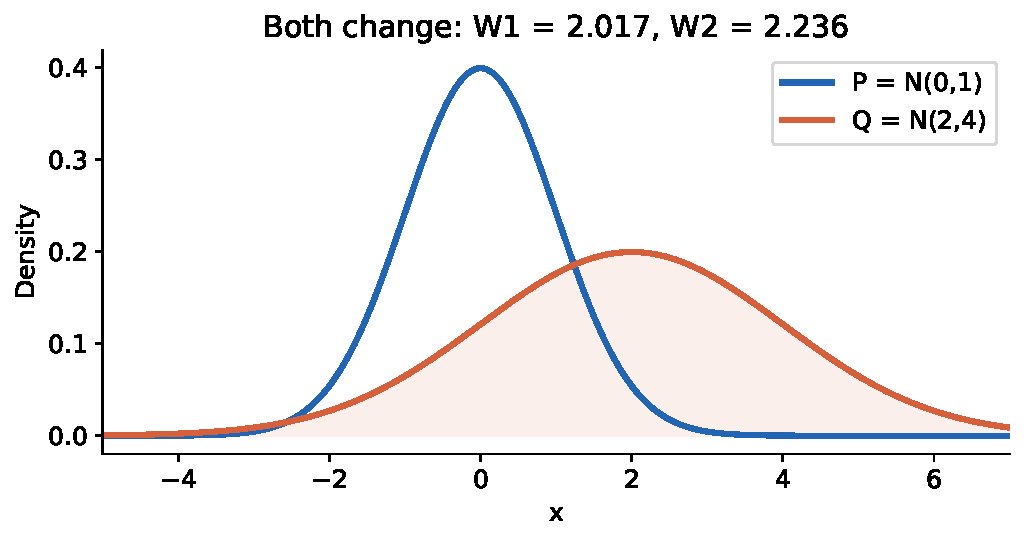
\includegraphics[width=\linewidth]{figures/gaussian_both.pdf}
\end{column}
\end{columns}
\vspace{2mm}
\small In general, put $m=|\mu_1-\mu_2|$, $s=|\sigma_1-\sigma_2|$. For $s>0$,
\[W_1=s\sqrt{2/\pi}\,e^{-m^2/(2s^2)}+m\big[2\Phi(m/s)-1\big].\]
If $s=0$, $W_1=m$. Here $\Phi$ is the standard normal CDF.
\end{frame}

% 16
\begin{frame}{Analytic distance and empirical computation}
\begin{itemize}\setlength\itemsep{3mm}
\item \textbf{Analytic:} derive a population formula from the assumed laws.
\item \textbf{Empirical:} replace the laws by weighted atoms at observed samples.
\item A computer can evaluate either a formula or an optimization problem.
\end{itemize}
\vspace{4mm}
\begin{center}\small\begin{tabular}{lrrrr}
\toprule
Change & Exact $W_1$ & Sample $W_1$ & Exact $W_2$ & Sample $W_2$\\
\midrule
Mean changes & 2.000 & 2.029 & 2.000 & 2.029\\
Variance changes & 0.798 & 0.809 & 1.000 & 1.006\\
Both change & 2.017 & 2.014 & 2.236 & 2.215\\
\bottomrule
\end{tabular}
\end{center}
\vspace{3mm}
Each row uses $4{,}000$ independently drawn samples per law, seed 2026.\\[2mm]
The empirical solver can be exact for its discrete inputs while its answer still has sampling error relative to the population distance.
\end{frame}

% 17
\begin{frame}[fragile]{Computing $W_1$ and $W_2$ by sorting}
\begin{lstlisting}[basicstyle=\ttfamily\footnotesize]
from scipy.stats import wasserstein_distance
import numpy as np

x = np.array([0., 1., 3.])
y = np.array([1., 2., 5.])
w1 = wasserstein_distance(x, y)
w2 = np.sqrt(np.mean((np.sort(x) - np.sort(y))**2))
\end{lstlisting}
Sorted displacements are $(1,1,2)$.
\[W_1=\frac{1+1+2}{3}=\frac43,\qquad W_2=\sqrt{\frac{1+1+4}{3}}=\sqrt2.\]
\alert{This $W_2$ code requires equal sample sizes and equal atom weights.}\\[2mm]
SciPy's \texttt{wasserstein\_distance} computes one-dimensional $W_1$ and also handles unequal sizes and supplied weights.
\src{https://docs.scipy.org/doc/scipy/reference/generated/scipy.stats.wasserstein_distance.html}{SciPy documentation: scipy.stats.wasserstein\_distance.}
\end{frame}

% 18
\begin{frame}{Discrete transport is a linear program}
\[P=\sum_{i=1}^{n}a_i\delta_{x_i},\qquad
Q=\sum_{j=1}^{m}b_j\delta_{y_j},\qquad \sum_i a_i=\sum_j b_j=1.\]
\[\boxed{W_p^p=\min_{\pi\geq0}\sum_{i,j}\pi_{ij}C_{ij}},\qquad
C_{ij}=\|x_i-y_j\|^p\]
\[\sum_j\pi_{ij}=a_i\quad\text{and}\quad\sum_i\pi_{ij}=b_j.\]
\begin{itemize}\setlength\itemsep{3mm}
\item Supports $x_i,y_j$ give locations. Weights $a_i,b_j$ give mass.
\item A dense cost matrix has $nm$ entries and becomes expensive for large images.
\item Numerical ``exact OT'' means unregularized optimization to solver tolerance.
\end{itemize}
\otref
\end{frame}

% 19
\begin{frame}[fragile]{A tiny weighted computation}
\begin{lstlisting}
x = np.array([0., 2.])
y = np.array([1., 3.])
a = np.array([.50, .50])
b = np.array([.25, .75])

w1 = wasserstein_distance(x, y, a, b)
w2, plan, cost = exact_ot(x, y, a, b, p=2)
\end{lstlisting}
\texttt{exact\_ot} in \texttt{ot\_tools.py} constructs the constraints and calls:
\begin{lstlisting}[basicstyle=\ttfamily\footnotesize]
result = linprog(cost.ravel(), A_eq=constraints,
                 b_eq=np.r_[a, b], bounds=(0, None), method="highs")
\end{lstlisting}
It checks convergence and both marginals before returning $W_p$, the plan, and costs.\\[2mm]
For histograms, pass bin locations as supports and counts as weights.
\src{https://docs.scipy.org/doc/scipy/reference/generated/scipy.optimize.linprog.html}{SciPy documentation: scipy.optimize.linprog. Full runnable implementation in ot\_tools.py.}
\end{frame}

% 20
\begin{frame}{Finite samples produce a nonzero baseline}
\fig[.80]{sampling}
\small
\begin{itemize}\setlength\itemsep{2mm}
\item Even independent samples from the same law usually have positive empirical distance.
\item Shading shows the 10th--90th percentiles across 80 repetitions, not confidence intervals.
\item Compare real/generated results with a real/real baseline at the same sample size.
\end{itemize}
\end{frame}

% 21
\begin{frame}{Sinkhorn adds entropy to the transport objective}
\[OT_\epsilon(P,Q)=\min_{\pi\in\Pi(P,Q)}
\sum_{ij}\pi_{ij}C_{ij}+\epsilon\sum_{ij}\pi_{ij}(\log\pi_{ij}-1).\]
\begin{itemize}\setlength\itemsep{3mm}
\item $\epsilon>0$ encourages mass to spread across more pairs.
\item With $K_{ij}=e^{-C_{ij}/\epsilon}$, the plan has form $\operatorname{diag}(u)K\operatorname{diag}(v)$.
\item Updates $u=a/(Kv)$ and $v=b/(K^\top u)$ enforce the marginals.
\end{itemize}
\vspace{2mm}
Our implementation uses log-space updates and checks marginal errors.\\[2mm]
The transport cost $\langle\pi_\epsilon,C\rangle$, the full objective $OT_\epsilon$, and exact $W_p^p$ are different quantities.
\src{https://arxiv.org/abs/1306.0895}{Cuturi (2013), Sinkhorn Distances. See notebook for log-domain implementation.}
\end{frame}

% 22
\begin{frame}{Regularization changes the optimal plan}
\fig[.86]{sinkhorn}
\vspace{-3mm}
\begin{center}\footnotesize\begin{tabular}{rrrr}
\toprule
$\epsilon$ & Transport cost & Full objective & $S_\epsilon$\\
\midrule
0.200 & 5.340 & 4.735 & 5.196\\
0.700 & 5.397 & 3.201 & 5.015\\
2.000 & 5.708 & -1.073 & 4.865\\
\bottomrule
\end{tabular}
\end{center}
\small Squared Euclidean cost. The debiased comparison subtracts self terms:
\[S_\epsilon(P,Q)=OT_\epsilon(P,Q)-\tfrac12OT_\epsilon(P,P)-\tfrac12OT_\epsilon(Q,Q).\]
\src{https://proceedings.mlr.press/v89/feydy19a.html}{Feydy et al. (2019), Sinkhorn divergences. S epsilon uses full regularized objectives with the same convention.}
\end{frame}

% 23
\begin{frame}{Two images can define different probability measures}
\fig[.94]{images}
\begin{itemize}\setlength\itemsep{2mm}
\item \textbf{Intensity distribution:} a random pixel's brightness. Here $W_1=0$.
\item \textbf{Spatial mass:} normalized brightness at pixel coordinates. Here $W_1=W_2=3$ pixels.
\item Both answers are correct for their chosen representation.
\end{itemize}
\end{frame}

% 24
\begin{frame}[fragile]{Computing spatial transport between tiny images}
\begin{lstlisting}[basicstyle=\ttfamily\footnotesize]
A = np.zeros((7, 7)); A[2:4, 1:3] = 1
B = np.zeros((7, 7)); B[2:4, 4:6] = 1
xy_a, mass_a = image_measure(A)
xy_b, mass_b = image_measure(B)
w1, plan, cost = exact_ot(xy_a, xy_b, mass_a, mass_b, p=1)
\end{lstlisting}
Each nonzero pixel carries mass $1/4$. Moving each pixel three columns right costs $3$.\\[3mm]
The mean horizontal position also shifts by $3$, so no plan can cost less.
\[\boxed{W_1=3\ \text{pixels}}\]
\small Normalization removes total brightness. Nonnegative intensities and positive total mass are required. Whole-image feature distributions answer a different question again.
\end{frame}

% 25
\begin{frame}{A value histogram loses time-series order}
\[A=(0,0,1,1),\qquad B=(0,1,0,1).\]
\fig[.91]{time_series}
\small Both amplitude distributions are $\frac12\delta_0+\frac12\delta_1$, so amplitude $W_1=0$.\\[2mm]
Including time coordinates changes the representation and the answer.
\end{frame}

% 26
\begin{frame}[fragile]{Transport between time-amplitude point clouds}
Give each observation mass $1/4$ at $(\lambda t_i,x_i)$.
\[d\big((t,x),(s,y)\big)=\sqrt{\lambda^2(t-s)^2+(x-y)^2}.\]
\begin{lstlisting}[basicstyle=\ttfamily\footnotesize]
t = np.arange(4)
A = np.array([0., 0., 1., 1.])
B = np.array([0., 1., 0., 1.])
cloud_a = np.c_[1.0*t, A]
cloud_b = np.c_[1.0*t, B]
w1, plan, cost = exact_ot(cloud_a, cloud_b)
\end{lstlisting}
At $\lambda=1$, $W_1=0.5$. At $\lambda=0$, the amplitude distance is $0$.\\[3mm]
The scale $\lambda$ specifies the time/amplitude tradeoff. This transport permits arbitrary pairings and does not enforce chronological alignment.
\end{frame}

% 27
\begin{frame}{Windows and whole paths preserve different information}
\textbf{Windows of length two}
\[A:\ (0,0),(0,1),(1,1),\qquad B:\ (0,1),(1,0),(0,1).\]
Their empirical $W_1$ with Euclidean ground distance is $2/3$.\\[4mm]
\textbf{Many complete time series}\\[2mm]
One path is one vector $x=(x_1,\ldots,x_T)$. For example,
\[d(x,y)=\sqrt{\frac1T\sum_{t=1}^T(x_t-y_t)^2}.\]
Transport compares a collection of real paths with a collection of generated paths.\\[3mm]
\small Windows retain local order. Whole-path vectors retain the chosen time grid. Overlapping windows are dependent, which matters for statistical testing.
\end{frame}

% 28
\begin{frame}{Signatures provide another representation of paths}
\begin{columns}
\begin{column}{.44\textwidth}
Embed a series as a path $(t,x_t)$.\\[2mm]
The notebook computes ordinary signature levels 1 through 3.\\[3mm]
Levels 1 and 2 agree here. At level 3:
\[S^{ttx}_A=7/54,\quad S^{ttx}_B=13/54.\]
OT or MMD can compare these feature distributions.
\end{column}
\begin{column}{.54\textwidth}
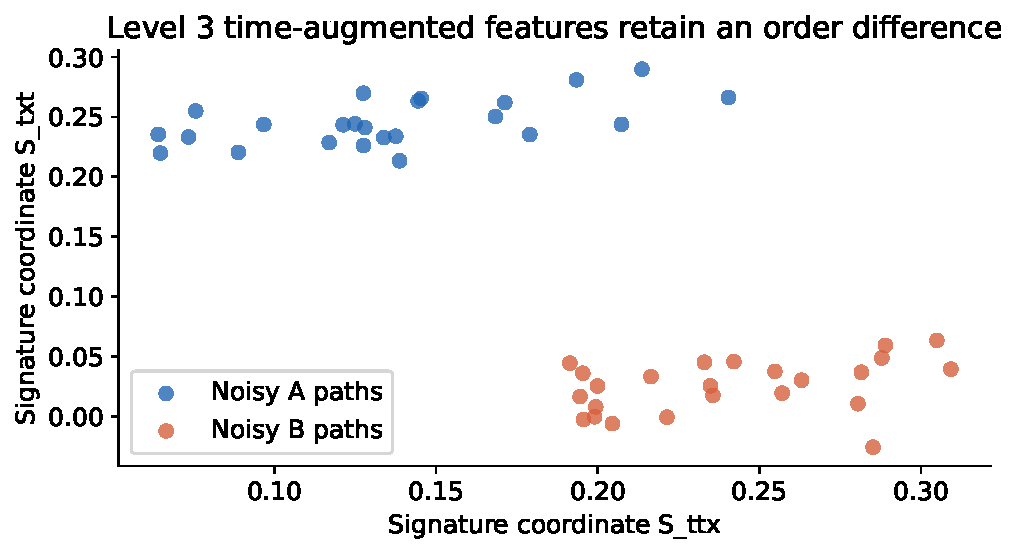
\includegraphics[width=\linewidth]{figures/signatures.pdf}
\end{column}
\end{columns}
\vspace{3mm}
\small Adding time can expose order. A scalar path's ordinary signature alone depends only on its total increment. Truncation loses information. These are not Volterra signatures.
\src{https://arxiv.org/abs/1603.03788}{Chevyrev and Kormilitzin, A Primer on the Signature Method in Machine Learning.}
\end{frame}

% 29
\begin{frame}{Maximum mean discrepancy compares kernel averages}
For independent copies $X,X'\sim P$ and $Y,Y'\sim Q$,
\[\mathrm{MMD}^2(P,Q)=\mathbb E k(X,X')+\mathbb E k(Y,Y')-2\mathbb E k(X,Y).\]
A common choice is the Gaussian kernel:
\[k(x,y)=\exp\!\left(-\frac{\|x-y\|^2}{2\ell^2}\right).\]
\begin{itemize}\setlength\itemsep{3mm}
\item The bandwidth $\ell$ controls which differences are emphasized.
\item For this characteristic kernel, population MMD is zero exactly when the input laws agree.
\item MMD compares kernel mean embeddings and does not return a transport plan.
\end{itemize}
\small The notebook reports biased empirical \textbf{MMD squared}, including diagonal kernel terms. Its finite-sample baseline can be positive.
\src{https://jmlr.org/papers/v13/gretton12a.html}{Gretton et al. (2012), A Kernel Two-Sample Test.}
\end{frame}

% 30
\begin{frame}[fragile]{MMD sensitivity depends on kernel bandwidth}
\fig[.83]{mmd}
\vspace{-2mm}
\begin{lstlisting}[basicstyle=\ttfamily\footnotesize]
score = mmd2_biased(real_features, generated_features, bandwidth=1.0)
\end{lstlisting}
\small Using scalar amplitudes for $A$ and $B$ still gives MMD $=0$. A different comparison rule cannot recover order discarded by the representation.\\[2mm]
The unbiased estimator excludes within-sample diagonals and can be negative.
\end{frame}

% 31
\begin{frame}{Which comparison answers the scientific question?}
\small
\begin{tabular}{>{\raggedright\arraybackslash}p{.18\textwidth}>{\raggedright\arraybackslash}p{.30\textwidth}>{\raggedright\arraybackslash}p{.42\textwidth}}
\toprule
Method & What it compares & Important choice or limitation\\\midrule
Wasserstein & Minimum transport cost & Ground distance, representation, $p$, sampling error\\[3mm]
MMD & Kernel mean embeddings & Kernel and bandwidth, feature information\\[3mm]
KL divergence & Relative probability density & Directional, can be infinite for disjoint support\\[3mm]
Aligned RMS & Values at corresponding times & Requires a shared time grid and alignment\\[3mm]
Dynamic time warping & Sequence alignment cost & Local cost and warping constraints, generally not a metric\\\bottomrule
\end{tabular}
\par\vspace{3mm}
Choose the representation first. Scores from different methods have different meanings.
\end{frame}

% 32
\begin{frame}{Connections to generative models}
\textbf{Wasserstein GANs} use the dual formulation
\[W_1(P,Q)=\sup_{\|f\|_{\rm Lip}\leq1}\big(\mathbb E_P f-\mathbb E_Q f\big).\]
A trained critic approximates this optimization under a Lipschitz constraint. The earlier ordinary GAN lesson does not implement WGAN.\\[4mm]
\textbf{Image evaluation:} FID applies a squared Gaussian $W_2$ formula to fitted image-feature distributions. It is not exact OT between raw image laws.\\[4mm]
\textbf{Flow matching:} learning a map between distributions does not by itself guarantee minimum transport cost.\\[3mm]
\small For generated time series, evaluate the path representation and temporal behavior, not only amplitude histograms.
\src{https://proceedings.mlr.press/v70/arjovsky17a.html}{Arjovsky et al. (2017), WGAN. FID: Heusel et al. (2017), arXiv:1706.08500.}
\end{frame}

% 33
\begin{frame}{A reproducible comparison workflow}
\begin{enumerate}\setlength\itemsep{4mm}
\item Specify one sample: a value, pixel location, window, whole path, or feature vector.
\item Define weights, coordinate units, normalization, and ground distance or kernel.
\item Use an analytic formula, 1D sorting, discrete OT, or a stated approximation.
\item Check a case with a known answer and check transport marginals.
\item Compare real/generated with real/real at matched sample sizes. Repeat across seeds.
\end{enumerate}
\vspace{3mm}
\small High dimension increases both computational and statistical difficulty. The included tiny LP is for learning, not full-resolution image processing.
\end{frame}

% 34
\begin{frame}{Exercises and predictions}
\begin{enumerate}\setlength\itemsep{4mm}
\item For $\mathcal N(0,1)$ and $\mathcal N(0,9)$, predict $W_1$ and $W_2$ before sampling.
\item Move the image patch two columns and one row. Predict spatial $W_1$ and intensity $W_1$.
\item Multiply every pixel intensity by $10$. What does normalization remove?
\item Permute a time series. Compare amplitudes, windows, whole paths, and signature features.
\item Increase Sinkhorn's $\epsilon$ or MMD's bandwidth. Which parts of the answer change?
\end{enumerate}
\vspace{3mm}
\small Run \texttt{learning\_wasserstein.ipynb}. Worked answers and teaching notes accompany the notebook in \texttt{README.txt}.
\end{frame}

% 35
\begin{frame}{References and further reading}
\small
\begin{itemize}\setlength\itemsep{2mm}
\item Peyr\'e and Cuturi. \href{https://arxiv.org/abs/1803.00567}{Computational Optimal Transport}. Foundations, Gaussian cases, algorithms.
\item \href{https://docs.scipy.org/doc/scipy/reference/generated/scipy.stats.wasserstein_distance.html}{SciPy: one-dimensional Wasserstein distance} and \href{https://pythonot.github.io/all.html}{POT: Python Optimal Transport}.
\item Cuturi (2013). \href{https://arxiv.org/abs/1306.0895}{Sinkhorn Distances}.
\item Feydy et al. (2019). \href{https://proceedings.mlr.press/v89/feydy19a.html}{Interpolating between OT and MMD using Sinkhorn Divergences}.
\item Gretton et al. (2012). \href{https://jmlr.org/papers/v13/gretton12a.html}{A Kernel Two-Sample Test}.
\item Chevyrev and Kormilitzin. \href{https://arxiv.org/abs/1603.03788}{A Primer on the Signature Method in Machine Learning}.
\item Arjovsky et al. (2017). \href{https://proceedings.mlr.press/v70/arjovsky17a.html}{Wasserstein Generative Adversarial Networks}.
\item Heusel et al. (2017). \href{https://arxiv.org/abs/1706.08500}{GANs Trained by a Two Time-Scale Update Rule} (FID).
\end{itemize}
\vspace{3mm}
All plotted data are synthetic examples generated by the accompanying code.
\end{frame}
\end{document}
